\documentclass[11pt]{beamer} % mathserif for normal math fonts.
\usefonttheme[onlymath]{serif}
\usepackage[utf8]{inputenc}
\usepackage[swedish,english]{babel}
\usepackage{microtype}
\usepackage{calc}
\usepackage{amsmath,mathtools}
\usepackage{contmech}
%\usepackage{subfig}
%\usepackage{siunitx}
%\usepackage{movie15}
\usepackage{wasysym}
\usepackage{multimedia}
\usepackage{grffile}
\usepackage{tikz}
\usepackage{pgfplots}

\pgfplotsset{compat=newest}
\usetikzlibrary{shapes,arrows}

\DeclarePairedDelimiter{\homgen}{\langle}{\rangle_\rve}
\DeclarePairedDelimiter{\shomgen}{\langle\!\langle}{\rangle\!\rangle_\rve}
\DeclarePairedDelimiter{\jmp}{[\![}{]\!]}
\newcommand{\jump}[1]{[\![#1]\!]}
\newcommand{\prescribed}{\mathrm{pre}}
\newcommand{\on}{\quad\text{ on }}
\renewcommand{\dev}{\mathrm{d}}
\renewcommand{\vol}{\mathrm{v}}
\newcommand{\per}{\mathrm{per}}
\newcommand{\volume}{|\Omega_\rve|}
\newcommand{\ded}{\mathrm{d}}
\newcommand{\dep}{\mathrm{p}}
\newcommand{\Periodic}{\mathrm{P}}
\newcommand{\external}{\mathrm{ext}}
\newcommand{\surf}{\mathrm{s}}
\newcommand{\pore}{\mathrm{pore}}
\newcommand{\particle}{\mathrm{part}}
\newcommand{\devop}{\ts\epsilon_\dev}
\newcommand{\densinv}{\eta}
\newcommand{\dens}{\eta^{-1}}
\newcommand{\epspargs}{\{{\bar{\ts d}}_\dev, \bar{p}\}}
\newcommand{\rve}{
  {\mathchoice
   {\mbox{\scalebox{0.67}{$\Box$}}}
   {\mbox{\scalebox{0.67}{$\Box$}}}
   {\mbox{\scalebox{0.5}{$\Box$}}}
   {\mbox{\scalebox{0.375}{$\Box$}}}
  }
}
%\usepgfplotslibrary{patchplots}
%\usepgfplotslibrary{groupplots}
%\pgfplotsset{compat=1.3}

\newcommand{\roughcite}[1]{\textsc{#1}}
\renewcommand{\alert}[1]{\textbf{#1}}

\setbeamersize{text margin left=.3cm,text margin right=.3cm}

\usetheme[titleflower=true]{chalmers}
\title{
On computational modeling of sintering based on homogenization
}
\author[Mikael \"Ohman --- 2014]{Mikael \"Ohman\\ Supervisors:\\ Kenneth Runesson \\ Fredrik Larsson}
\institute{Department of Applied Mechanics\\ Chalmers University of Technology\\
mikael.ohman@chalmers.se
}
%\titlepageextra{2012}% session: Multiple-scale physics and computation
\date{2014-06-13}
%\footer{\insertshortauthor\ 2\textsuperscript{nd} ICMM}
\titlepagelogofile{Avancez_black}

% Bibliography
%\bibliography{references_extended}

% Speeds up compilation.
% \usetikzlibrary{external}
% \tikzexternalize



\begin{document}

\section{Title page}
\begin{frame}[plain]
 \titlepage
\end{frame}

\section{Preface}
\begin{frame}
 \frametitle{Preface}
 \begin{center}
 Swedish Research Council (Vetenskapsrådet)
 \\[2em]
 Supervisors:\\
 Professor Kenneth Runesson \\
 Professor Fredrik Larsson
 \end{center}
\end{frame}

\section{Outline}
\begin{frame}
 \frametitle{Outline}

\begin{itemize}
 \item Motivation of project / background on sintering
 \item Classical (macroscale) constitutive modeling of sintering
 \item Fine scale problem
 \item Two-scale problem:
 \begin{itemize}
  \item Paper A ---
  \item Paper B --- 
  \item Paper C --- 
  \item Paper D ---  
 \end{itemize}
 \item Conclusions
 \item Outlook
\end{itemize}
\end{frame}


% \section{Background}
% %%%%%%%%%%%%%%%%%%%%%%%%%%%%%%%%%%%%%%%%%%%%%%%%%%%%%%%%%%%%%%%%%%%%%%%%%%%%%%%%%%%%%%%%%%%%%%%%%%%
% \begin{frame}
%  \frametitle{Research project}
%  \begin{itemize}
%   \item PhD project funded by the Swedish research council
%   \item Supervisors Prof. Kenneth Runesson and Prof. Fredrik Larsson
%   \item Expected to be finished in 2014
%  \end{itemize}
% \end{frame}

%%%%%%%%%%%%%%%%%%%%%%%%%%%%%%%%%%%%%%%%%%%%%%%%%%%%%%%%%%%%%%%%%%%%%%%%%%%%%%%%%%%%%%%%%%%%%%%%%%%
\section{Background}
\begin{frame}
 \frametitle{Motivation --- Sintering of hardmetal}

% The sintering phenomenon on the mesoscale is driven by surface tension on the melted binder, and
% the homogenized effect of the surface tension is the so-called sintering stress.
% From the macroscopic perspective, the specimen (green body) shrinks due to this volumetric sintering stress. In the case of inhomogeneous
% initial density in the green body, the sintering can result in unwanted final deformations.

 \begin{enumerate}
  \item WC-particles in Co-matrix (binder metal)
  \item Precompaction $\rightarrow$ inhomogeneous ``green body'', porosity $\phi_0\approx$ 0.2--0.4
  \item Heating $\rightarrow$ thermal expansion, sintering driven by surface tension in melted Co, i.e. ``liquid phase sintering'' $\rightarrow$
        Fully dense final product $\phi=0$.
 \end{enumerate}
\alert{Note:} Inhomogeneous initial density may lead to defect product:\\ \textsuperscript{(i)}remaining porosity, \textsuperscript{(ii)}shape imperfection\\
\alert{Note:} Macroscopic compressibility despite \underline{assumed} intrinsic incompressibility of constituents until $\phi = 0$.
\begin{center}
 \begin{columns}
 \column{0.25\textwidth}\centering
 \begin{tikzpicture}
   \node at (0,0) {\includegraphics[width=\textwidth]{figures/sinter_1-crop.pdf}};
   \draw[red,thick,<-] (1,1) -- (1.5,1) node[right,black] {WC};
   \draw[red,thick,<-] (0.5,0.7) -- (1.5,0.5) node[right,black] {Co};
   \draw[red,thick,<-] (0.7,-0.3) -- (1.5,0) node[right,black] {pore};
 \end{tikzpicture}
 \column{0.05\textwidth}\centering
 $\xrightarrow{\text{idealized}}$
 \column{0.25\textwidth}\centering
 \includegraphics[width=\textwidth]{figures/sinter_2-crop.pdf}
 \end{columns}
 %\includegraphics[width=0.6\textwidth]{figures/fig081.jpeg}
\end{center}
\end{frame}


%%%%%%%%%%%%%%%%%%%%%%%%%%%%%%%%%%%%%%%%%%%%%%%%%%%%%%%%%%%%%%%%%%%%%%%%%%%%%%%%%%%%%%%%%%%%%%%%%%%
\begin{frame}
 \frametitle{Motivation --- Green body}

% The sintering phenomenon on the mesoscale is driven by surface tension on the melted binder, and
% the homogenized effect of the surface tension is the so-called sintering stress.
% From the macroscopic perspective, the specimen (green body) shrinks due to this volumetric sintering stress. In the case of inhomogeneous
% initial density in the green body, the sintering can result in unwanted final deformations.

 \begin{itemize}
  \item Green body: Compacted (metal) powder
  %\includegraphics[]{figures/}
  \begin{tikzpicture}
  \node at (0,0) {\includegraphics[scale=1.0]{figures/GreenBody.pdf}};
  \draw[latex-] (-2.8,0.1) -- ++(-1,0) node[left] {$\Omega^\particle$};
  \draw[latex-] (-2.8,-0.35) to (-3.8,0.1);
  \draw[-] (3.1,0) -- ++(1,0) node[right] {$\Gamma$};
  \draw[<-] (1.42,0.6) -- (4.1,0.6) node[right] {$\Gamma^\pore$};
  \end{tikzpicture}
  %\caption{Green body with its macroscopic shape as dashed line. Particles are not to scale.}
  \item To many particles to solve directly
 \end{itemize}
\end{frame}

%%%%%%%%%%%%%%%%%%%%%%%%%%%%%%%%%%%%%%%%%%%%%%%%%%%%%%%%%%%%%%%%%%%%%%%%%%%%%%%%%%%%%%%%%%%%%%%%%%%
\begin{frame}
 \frametitle{Constitutive modeling}
 Macroscopic modeling of sintering
 \begin{itemize}
  \item Typically porosity as an internal variable
  \item Complex model structure, requires many parameters --- calibration problem very ill-posed
  \item Selected references: \roughcite{Svoboda \& Riedel (1996)}, \roughcite{Mähler, Ekh \& Runesson (1999)}, \roughcite{Olevsky \& German (1998)}
 \end{itemize}

Mesoscale modeling - deformation driven by surface tension
 \begin{itemize}
  \item Multi-particle sintering
  \item Selected references: \roughcite{Jagota \& Dawson (1988)}, \roughcite{Xu \& Mehrabadi (1997)}, \roughcite{Zhou \& Derby (1998)}, \roughcite{Peric et al.\ (2006-)}, \roughcite{Javili \& Steinmann (2009)}, \roughcite{Pino-Muñoz et al.\ (2013)}
 \end{itemize}

% Computational homogenization - FE\textsuperscript{2}
% \begin{itemize}
%   \item Selected references:  \roughcite{Geers \& al.},  \roughcite{Fish \& al.},
%  \roughcite{Miehe \& al.}, \roughcite{Larsson \& Runesson [adaptive multiscale]}
% \end{itemize}
\end{frame}

%%%%%%%%%%%%%%%%%%%%%%%%%%%%%%%%%%%%%%%%%%%%%%%%%%%%%%%%%%%%%%%%%%%%%%%%%%%%%%%%%%%%%%%%%%%%%%%%%%%
\section{Theory}
% \begin{frame}
%  \frametitle{Surface tension on free surface and interfaces}
% \small
%  \vspace{-1em}
%  \begin{center}
%   \scalebox{0.75}{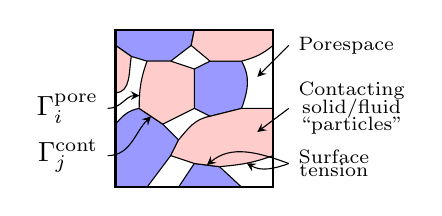
\begin{tikzpicture}[>=stealth,scale=2]
  \coordinate (A) at (0.35,0.2);
  \coordinate (B) at (0.4,0.3);
  \coordinate (C) at (0.3,0.4);
  \coordinate (D) at (0.15,0.5);
  \coordinate (E) at (0.66,0.13);
  \coordinate (F) at (0.6,0.45);
  \coordinate (G) at (0.8,0.5);
  \coordinate (H) at (0.5,0.5);
  \coordinate (I) at (0.5,0.75);
  \coordinate (J) at (0.6,0.8);
  \coordinate (K) at (0.8,0.8);
  \coordinate (L) at (0.35,0.8);
  \coordinate (M) at (0.5,1);
  \coordinate (N) at (0,0.9);
  \coordinate (O) at (0.1,0.83);
  \coordinate (P) at (0.5,0.15);
  \coordinate (Q) at (0.48,0.9);
  \coordinate (R) at (0.2,0.8);
  
  % Region 1 particles 
  \draw[fill=blue!40] 
  (0,0) -- (0.2,0) -- (A) -- (B) -- (C) -- (D) to[out=190,in=50] (0,0.4) -- cycle %A
  (0.4,0) -- (P) -- (E) -- (0.8,0) -- cycle %B
  (F) -- (G) to[out=70,in=-60] (K) -- (J) -- (I) -- (H) -- cycle %C
  (M) -- (Q) -- (L) -- (R) -- (O) -- (N) -- (0,1) -- cycle %D
  ;

  % Region 2 particles
  \draw[fill=red!20]
  (0,0.6) to[out=0,in=-100] (O) -- (N) -- cycle %E
  (D) to[out=90,in=-110] coordinate[near start] (surf3) (R) -- (L) -- (I) -- (H) -- (C) -- (D) coordinate[midway] (surf4) %F
  (M) -- (Q) -- (J) -- (K) to[out=15,in=-140] (1,0.9) -- (1,1) -- cycle %G
  (1,0.2) to[out=-160,in=5] coordinate[midway] (surf1) (E) -- (P) coordinate[midway] (surf2) -- (A) -- (B) to[out=50,in=-170] (F) -- (G) -- (1,0.5) -- cycle %H
  ;

  \draw[thick] (0,0) rectangle (1,1);

  % Annotations
  \draw[<-] (0.9,0.7) -- (1.1,0.9) node[right,font=\scriptsize] {Porespace};
  \draw[<-] (0.9,0.35) -- (1.1,0.5) node[right,font=\scriptsize] {\shortstack{Contacting\\[-0.4em]solid/fluid\\[-0.4em]``particles''}};
  \draw[<-] (surf1) to[out=-30,in=-160] (1.1,0.15) node[right,font=\scriptsize] {\shortstack{Surface\\[-0.4em]tension}};
  \draw[<-] (surf2) to[out=40,in=160] (1.1,0.15); % extra arrow
  \draw[<-] (surf3) to[out=180,in=0] (-0.05,0.5) node[left] {$\Gamma_i^{\mathrm{pore}}$};
  \draw[<-] (surf4) to[out=-135,in=0] (-0.05,0.2) node[left] {$\Gamma_j^{\mathrm{cont}}$};
\end{tikzpicture}}
%   \hspace{0.5em}
%   \scalebox{0.75}{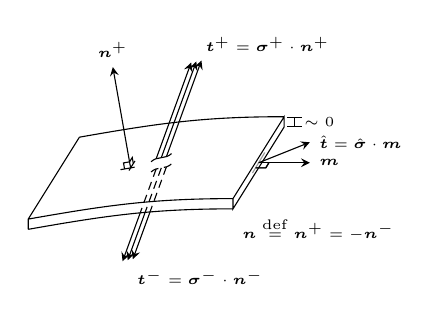
\begin{tikzpicture}[>=stealth,scale=1.3,font=\tiny]
 \coordinate (A) at (0,0);
 \coordinate (B) at (2,0.2);
 \coordinate (C) at (2.5,1);
 \coordinate (D) at (0.5,0.8);
 \coordinate (At) at (0,-0.1);
 \coordinate (Bt) at (2,0.1);
 \coordinate (Ct) at (2.5,0.9);

 \draw (A) to[out=10,in=180] (B)
      (At) to[out=10,in=180] (Bt)
      (Bt) -- (B) -- (C) coordinate[midway] (E) -- (Ct) -- cycle
      (At) -- (A) -- (D) to[out=10,in=180] (C);

 % Binormal m
 \draw[draw=black!40] (E)++(0,-0.05)++(-0.06,-0.1) -- +(0.12,0.2);
 \draw[->] (E)++(0,-0.05) -- +(0.5,0) node[right]{$\boldsymbol{m}$};
 \draw[->] (E)++(0,-0.05) -- +(0.5,0.2) node[right]{$\hat{\boldsymbol{t}}=\hat{\boldsymbol{\sigma}}\cdot\boldsymbol{m}$};
 \draw (E)++(-0.03,-0.1) -- ++(0.1,0) -- +(0.03,0.05);
 \draw (E)++(0,-0.05)++(-0.03,-0.05) -- ++(0.1,0) -- +(0.03,0.05);

 
 % Normal
 \coordinate (n) at (1,0.5);
 \draw[->] (n) -- +(100:1) node[above]{$\boldsymbol{n}^+$};
 \draw (n)++(190:0.06) -- ++(100:0.06) -- +(190:-0.06);
 \draw (n)++(190:0.1) -- +(190:-0.14);
 \draw (n)++(58:0.05) -- ++(100:0.06) -- +(58:-0.05);
 \draw (n)++(58:0.08) -- +(58:-0.11);
 %\draw (n)++(190:0.06) -- ++(58:0.05) -- ++(190:-0.06);
 
 % Traction +
 \draw[->] (1.3,0.6) -- +(70:1) node[above right]{$\boldsymbol{t}^+ = \boldsymbol{\sigma}^+\cdot\boldsymbol{n}^+$};
 \draw[->] (1.35,0.61) -- +(70:1);
 \draw[->] (1.25,0.59) -- +(70:1);
 \draw (1.2,0.56) to[out=45,in=-135] (1.4,0.64);

 % Traction -
 \draw[densely dashed] (1.3,0.5) -- +(-110:0.46) coordinate (tmin); \draw[->] (tmin) -- +(-110:0.5) node[below right]{$\boldsymbol{t}^- =  \boldsymbol{\sigma}^-\cdot\boldsymbol{n}^-$};
 \draw[densely dashed] (1.35,0.51) -- +(-110:0.46) coordinate (tmin); \draw[->] (tmin) -- +(-110:0.5);
 \draw[densely dashed] (1.25,0.49) -- +(-110:0.46) coordinate (tmin); \draw[->] (tmin) -- +(-110:0.5);
 \draw[densely dashed] (1.2,0.46) to[out=45,in=-135] (1.4,0.54);

 % Thickness
 \draw[|-|] ([xshift=0.1cm]C) -- ([xshift=0.1cm]Ct) node[midway,right] {$\sim 0$};

 % Definition
 \node[right] at (2,-0.1) {$\boldsymbol{n} \overset{\mathrm{def}}{=} \boldsymbol n^+ = -\boldsymbol n^-$};
\end{tikzpicture}}
%  \end{center}
% \vspace{-1em}
% \begin{itemize}
%  \item Equilibrium for tractions on smooth surface/interface segments
% \vspace{-0.7em}
% \begin{align*}
%  \ta t^+ + \ta t^- + \ta t_\surf = \ta 0 \text{ on } \Gamma_i^{\mathrm{pore}} \text{ or } \Gamma_j^{\mathrm{cont}},\quad \ta t_\surf \defeq \hat{\ts\sigma}\cdot\hat{\ta\nabla}
% \end{align*}
% $\hat{\ts\sigma} =$ ``surface stress'' (in tangent plane), $\hat{\ta\nabla} =$ ``surface \rlap{gradient''}
%  \item Particle/pore boundaries $\Gamma_i^{\mathrm{pore}}:\;\;\ta t\defeq \ts\sigma^-\cdot\ta n = \ta t_\surf$
% \item Special case: Isotropic homogeneous surface tension: $\hat{\ts\sigma}=\gamma_\surf \hat{\ta I}$, $\hat{\ts I}\defeq\ts I-\ta n\outerp\ta n$ \vspace{-0.5em}
% \begin{align*}
%  \implies\quad \ta t_\surf = - \kappa \gamma_s \ta n,\quad \kappa \defeq \ta n \cdot \hat{\ta\nabla} \text{ (curvature)}
% \end{align*}
%  %\item \roughcite{Steinmann, Javili \& Steinmann (2009-)}
% \end{itemize}
% \end{frame}

%%%%%%%%%%%%%%%%%%%%%%%%%%%%%%%%%%%%%%%%%%%%%%%%%%%%%%%%%%%%%%%%%%%%%%%%%%%%%%%%%%%%%%%%%%%%%%%%%%%
\begin{frame}
 \frametitle{Subscale constitutive modeling}
 \begin{itemize}
  \item Incompressible, viscous flow $\leadsto$ Stokes' flow.
  \begin{gather*}
   \ts\sigma_\dev = 2\mu {\ts d}_\dev\\
   \ts\sigma_\dev = \ts\sigma + p\ts I,\quad \ts d_\dev \defeq [\ts v\outerp \diff]_\dev^\sym
  \end{gather*}
  \item Particles: Approximated as incompressible viscous flow with large viscosity surrounded by binder with lower viscosity
  \begin{align*}
   \mu^{\mathrm{part}} > \mu^{\mathrm{binder}}
  \end{align*}
  \item Quasistatic motion of viscoplastic particles, spatial setting:
  \begin{align*}
   -\ts\sigma(\ts d)\cdot\ta\nabla = \ta 0 \text{ in } \Omega^\particle,\quad \ta v\cdot\ta\nabla = 0 \text{ in } \Omega^\particle%, \quad \Omega^\particle = \cup_\alpha \Omega_\alpha^\particle
  \end{align*}
  %\alert{Note}: Tangent ``stiffness'' $\tf E_{\mathrm{T},\dev}$ from $\dif\ts\sigma_\dev = \tf E_{\mathrm{T},\dev}\dprod \dif\ts d$ used in Newton iterations on subscale (RVE-problem)
 \end{itemize}
\end{frame}

%%%%%%%%%%%%%%%%%%%%%%%%%%%%%%%%%%%%%%%%%%%%%%%%%%%%%%%%%%%%%%%%%%%%%%%%%%%%%%%%%%%%%%%%%%%%%%%%%%%
\begin{frame}
 \frametitle{Surface tension}
%\begin{figure}[th!]
    \begin{center}
    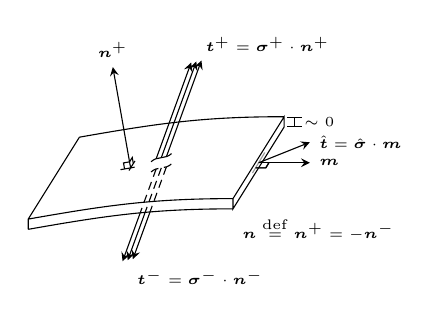
\begin{tikzpicture}[>=stealth,scale=1.3,font=\tiny]
 \coordinate (A) at (0,0);
 \coordinate (B) at (2,0.2);
 \coordinate (C) at (2.5,1);
 \coordinate (D) at (0.5,0.8);
 \coordinate (At) at (0,-0.1);
 \coordinate (Bt) at (2,0.1);
 \coordinate (Ct) at (2.5,0.9);

 \draw (A) to[out=10,in=180] (B)
      (At) to[out=10,in=180] (Bt)
      (Bt) -- (B) -- (C) coordinate[midway] (E) -- (Ct) -- cycle
      (At) -- (A) -- (D) to[out=10,in=180] (C);

 % Binormal m
 \draw[draw=black!40] (E)++(0,-0.05)++(-0.06,-0.1) -- +(0.12,0.2);
 \draw[->] (E)++(0,-0.05) -- +(0.5,0) node[right]{$\boldsymbol{m}$};
 \draw[->] (E)++(0,-0.05) -- +(0.5,0.2) node[right]{$\hat{\boldsymbol{t}}=\hat{\boldsymbol{\sigma}}\cdot\boldsymbol{m}$};
 \draw (E)++(-0.03,-0.1) -- ++(0.1,0) -- +(0.03,0.05);
 \draw (E)++(0,-0.05)++(-0.03,-0.05) -- ++(0.1,0) -- +(0.03,0.05);

 
 % Normal
 \coordinate (n) at (1,0.5);
 \draw[->] (n) -- +(100:1) node[above]{$\boldsymbol{n}^+$};
 \draw (n)++(190:0.06) -- ++(100:0.06) -- +(190:-0.06);
 \draw (n)++(190:0.1) -- +(190:-0.14);
 \draw (n)++(58:0.05) -- ++(100:0.06) -- +(58:-0.05);
 \draw (n)++(58:0.08) -- +(58:-0.11);
 %\draw (n)++(190:0.06) -- ++(58:0.05) -- ++(190:-0.06);
 
 % Traction +
 \draw[->] (1.3,0.6) -- +(70:1) node[above right]{$\boldsymbol{t}^+ = \boldsymbol{\sigma}^+\cdot\boldsymbol{n}^+$};
 \draw[->] (1.35,0.61) -- +(70:1);
 \draw[->] (1.25,0.59) -- +(70:1);
 \draw (1.2,0.56) to[out=45,in=-135] (1.4,0.64);

 % Traction -
 \draw[densely dashed] (1.3,0.5) -- +(-110:0.46) coordinate (tmin); \draw[->] (tmin) -- +(-110:0.5) node[below right]{$\boldsymbol{t}^- =  \boldsymbol{\sigma}^-\cdot\boldsymbol{n}^-$};
 \draw[densely dashed] (1.35,0.51) -- +(-110:0.46) coordinate (tmin); \draw[->] (tmin) -- +(-110:0.5);
 \draw[densely dashed] (1.25,0.49) -- +(-110:0.46) coordinate (tmin); \draw[->] (tmin) -- +(-110:0.5);
 \draw[densely dashed] (1.2,0.46) to[out=45,in=-135] (1.4,0.54);

 % Thickness
 \draw[|-|] ([xshift=0.1cm]C) -- ([xshift=0.1cm]Ct) node[midway,right] {$\sim 0$};

 % Definition
 \node[right] at (2,-0.1) {$\boldsymbol{n} \overset{\mathrm{def}}{=} \boldsymbol n^+ = -\boldsymbol n^-$};
\end{tikzpicture}
    %\caption{Thin shell representing a surface with in-plane forces due to ``surface tension''.}
    %\label{fig:surfacestress}
    \end{center}
%\end{figure}
% A vital part of the simulation is the modeling of surface tension, which acts as the ``driving force'' for liquid-phase sintering.
% An extensive theory on boundary energy potentials has been developed by Steinmann \cite{steinmann_boundary_2008}, which has served as the basis for the surface tension modeling in this work.
% In short; equilibrium across a surface $\mathcal{S}$ represented by a thin shell bounded by the curve $\mathcal{C}$, as in \figref{fig:surfacestress}, can be stated as:
\begin{align}
    \ta{t}^+ + \ta{t}^- + \ta{t}_\surf &= \ta{0} \quad \text{on} \,\, \mathcal{S} \quad \text{with } \ta{t}_\surf \defeq \hat{\ts\sigma}\cdot\hat{\diff}
\label{eq103KR}\\
    \sum_i \hat{\ta t}_i &= \ta{0} \quad \text{on} \,\, \mathcal{C}
\label{eq104KR}
\end{align}
where $\hat\diff \defeq \diff - [\diff\cdot\ta n]\ta n$.
Only isotropic surface tension considered: $\hat{\ts\sigma} = \gamma_\surf[\ts I-\ta n\outerp\ts n]$ $\implies$
$ \ta t_\surf = -\kappa \gamma_\surf \ta n$, where $\kappa \defeq \ta n \cdot\hat{\diff}$.
\end{frame}

%%%%%%%%%%%%%%%%%%%%%%%%%%%%%%%%%%%%%%%%%%%%%%%%%%%%%%%%%%%%%%%%%%%%%%%%%%%%%%%%%%%%%%%%%%%%%%%%%%%
\begin{frame}
 \frametitle{Weak form of ``fine-scale'' problem}
%\footnotesize
 \begin{itemize}
  \item Sintering particles occupying domain $\Omega^\particle$ with internal pore boundary $\Gamma^\pore$:
Find $(\ta v,p)\in \set V \times \set P$ such that
\begin{align*}
  \int_{\mathrlap{\Omega^\particle}} \;\ts\sigma\dprod[\delta\ta v\outerp\ta\nabla]\dif v &=
   \int_{\mathrlap{\Gamma^\pore}} \;\gamma_\surf[\delta\ta v\cdot\hat{\ta\nabla}] \dif a +
    \int_{\mathrlap{\Gamma_\Neumann^\external}} \;\ta t_p\cdot\delta\ta v\dif a \; && \forall \delta \ta v\in \set V^0\\
  \int_{\mathrlap{\Omega^\particle}} \;[\ta v\cdot\ta\nabla]\delta p\dif v &= 0 && \forall \delta p\in \set P
\end{align*}
%\alert{Note}: Obtained via use of surface divergence theorem + equilibrium for singular curves $C_i$

 \item \alert{Surface tension}: Stems from the surface potential, defined by $\gamma_\surf$.
 \item \alert{Remark}: Incompressible elasticity in Paper D: replace $\ta v \to \ta u$
 \end{itemize}
\end{frame}


%%%%%%%%%%%%%%%%%%%%%%%%%%%%%%%%%%%%%%%%%%%%%%%%%%%%%%%%%%%%%%%%%%%%%%%%%%%%%%%%%%%%%%%%%%%%%%%%%%%
\begin{frame}
 \frametitle{Two-scale problem}

\begin{figure}[htpb!]
\centering
\scalebox{0.75}{
\begin{tikzpicture}[scale=1.0]
 \node at (0,0) {\includegraphics[scale=0.6]{figures/Homogenization}};
 \draw[-] (1.35,1.5) -- +(-0.5,0) node[left] {$\Omega_\rve$};
 \node at (2.5,1.5) {RVE};
 \node at (-2.5,-2.2) {Fine-scale};
 \node at (2.5,-2.2) {Macroscale};
 \node at (0,0) {VCH};
 \draw[latex-] (-4.1,0.1) -- ++(-1,0) node[left] {$\Omega^\particle$};
 \draw[latex-] (-4.2,-0.15) to (-5.1,0.1);
 \draw[latex-] (4.4,0) -- ++(1,0) node[right] {$\Gamma^\Neumann$, $\Gamma^\Dirichlet$};
 \node at (2.5,-0.5) {$\Omega$};
\end{tikzpicture}
}
\caption{Homogenization of a ``green body''}
\label{fig:homogenization}
\end{figure}
% 
\begin{figure}[htpb!]
\centering
\scalebox{0.75}{
\begin{tikzpicture}[scale=1.0]
 \node at (0,0) {\includegraphics[scale=0.15]{figures/initial_rve}};
 \node at (-0.75,0.85) {$\Omega_\rve^\particle$};
 \draw[latex-] (-1.33,0.) -- ++(-1,0) node[left] {$\Gamma_\rve$};
 \draw[latex-] (45:0.5) -- +(1.6,0.5) node[right] {$\Gamma_\rve^\pore$};
\end{tikzpicture}
}
\caption{Idealized RVE consisting of a single unit cell of spherical particles in contact.}
\label{fig:rve_example}
\end{figure}
\end{frame}



%%%%%%%%%%%%%%%%%%%%%%%%%%%%%%%%%%%%%%%%%%%%%%%%%%%%%%%%%%%%%%%%%%%%%%%%%%%%%%%%%%%%%%%%%%%%%%%%%%%
%%%%%%%%%%%%%%%%%%%%%%%%%%%%%%%%%%%%%%%%%%%%%%%%%%%%%%%%%%%%%%%%%%%%%%%%%%%%%%%%%%%%%%%%%%%%%%%%%%%
%%%%%%%%%%%%%%%%%%%%%%%%%%%%%%%%%%%%%%%%%%%%%%%%%%%%%%%%%%%%%%%%%%%%%%%%%%%%%%%%%%%%%%%%%%%%%%%%%%%
%%%%%%%%%%%%%%%%%%%%%%%%%%%%%%%%%%%%%%%%%%%%%%%%%%%%%%%%%%%%%%%%%%%%%%%%%%%%%%%%%%%%%%%%%%%%%%%%%%%
%%%%%%%%%%%%%%%%%%%%%%%%%%%%%%%%%%%%%%%%%%%%%%%%%%%%%%%%%%%%%%%%%%%%%%%%%%%%%%%%%%%%%%%%%%%%%%%%%%%
%%%%%%%%%%%%%%%%%%%%%%%%%%%%%%%%%%%%%%%%%%%%%%%%%%%%%%%%%%%%%%%%%%%%%%%%%%%%%%%%%%%%%%%%%%%%%%%%%%%


\section{Paper}
\subsection{A}
\begin{frame}
 \frametitle{Paper A}
\begin{center}
 %\fullcite{ohman_computational_2012}
\end{center}
\end{frame}

\subsection{B}
\begin{frame}
 \frametitle{Paper B}
\begin{center}
 %\fullcite{ohman_computational_2013}
\end{center}
\end{frame}

\subsection{C}
\begin{frame}
 \frametitle{Paper C}
\begin{center}
 %\fullcite{ohman_variationally_2014}
\end{center}
\end{frame}

\subsection{D}
\begin{frame}
 \frametitle{Paper D}
\begin{center}
 %\fullcite{ohman_new_2014}
\end{center}
\end{frame}


% \subsection{Classical Homogenization}
% %%%%%%%%%%%%%%%%%%%%%%%%%%%%%%%%%%%%%%%%%%%%%%%%%%%%%%%%%%%%%%%%%%%%%%%%%%%%%%%%%%%%%%%%%%%%%%%%%%%
% \begin{frame}
%  \frametitle{RVE-problem}
% \begin{itemize}
%  \item Homogenization on Representative Volume Element (RVE) occupying bulk volume $\Omega_\Box$ with external boundary $\Gamma_\Box$
%  \begin{align*}
%   \int_{\Omega^{\mathrm{part}}} f \dif v \stackrel{\text{replaced by}}{\to} \int_\Omega \langle f\rangle_\Box \dif \bar{v}, \quad \langle f\rangle_\Box \defeq \frac1{|\Omega_\Box|} \int_{\Omega_\Box^{\mathrm{part}}} f \dif v
%  \end{align*}
%  \item 2D-RVE with single unit cell (example): Initially perfect square lattice. Contact surfaces are initially flattened from precompaction.
% \end{itemize}
%  \begin{center}
%   \begin{columns}
%    \column{0.2\textwidth}
%    \column{0.3\textwidth}\centering
%     \resizebox{!}{0.8\textwidth}{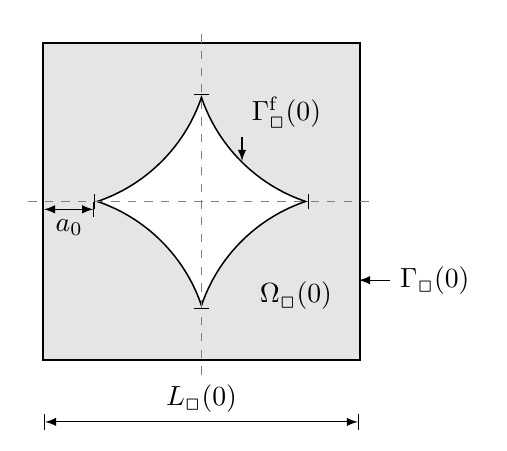
\begin{tikzpicture}[>=latex,scale=2] % Use this to scale the image. Text is always normal-size
  \def\particleradius{1.05} % Adjust this to change the contact size.
  \pgfmathsetmacro{\contactsize}{sqrt(\particleradius^2-1)} % Automatically calculated.
  \begin{scope}[very thick]
  	\draw[clip] (-1,-1) rectangle (1,1);
  	\draw[clip]
  		(-1,-1) circle (\particleradius)
 		( 1,-1) circle (\particleradius)
 		(-1, 1) circle (\particleradius)
   		( 1, 1) circle (\particleradius);
  	\fill[fill=black!10] (-1,-1) rectangle (1,1);
  \end{scope}
  % Markers
  \foreach \q in {0,90,180,270} { \draw[rotate=\q] (1-\contactsize,-0.05) -- +(0,0.1); }
  \draw[dashed,gray] (-1.1,0) -- (1.1,0) (0,-1.1) -- (0,1.1);
  % Annotations
  %\node[below] at (0,0) {$\Omega_\Box^p(0)$};
  \draw[|<->|] (-1,-1.4) -- (1,-1.4) node[midway,above] {$L_\Box(0)$};
  \draw[<->|] (-1,-0.05) -- +(\contactsize,0) node[midway,below] {$a_0$};
  \node at (0.6,-0.6) {$\Omega_\Box(0)$};
  \draw[<-] (1,-0.5) -- +(0.2,0) node[right] {$\Gamma_\Box(0)$};
  \draw[<-] (1,1) ++(-135:\particleradius) -- +(0.00,0.15) node[above right] {$\Gamma_\Box^{\mathrm{f}}(0)$};
  
  %\draw[use as bounding box] (-1.7,-1.5) rectangle (1.7,1.1);
  %\useasboundingbox (-1.7,-1.5) (1.7,1.1);
  % Transformation arrow (makes the picture very unaligned)
  %\draw[->] (1.5,0) to[out=45,in=-150] (2,0);% +(135:0.1) -- (2,0) -- +(-135:0.1);
\end{tikzpicture}
}
%    %\column{0.3\textwidth}\centering
%    % \resizebox{!}{0.8\textwidth}{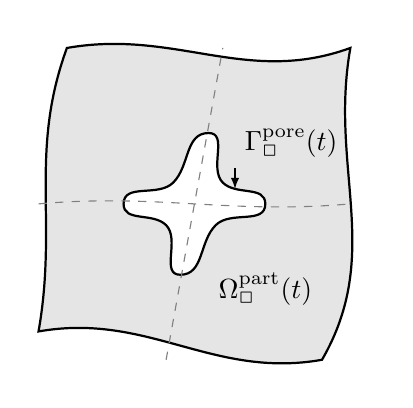
\begin{tikzpicture}[>=latex,scale=1.8] % Use this to scale the image. Text is always normal-size
  \def\particleradius{1.05} % Adjust this to change the contact size.
  \draw[thick,fill=black!10,even odd rule] (0.9,-1.1) 
  	to[out=190,in=10] (-1.1,-0.9)
  	to[out=80,in=-110] (-0.9,1.1)
  	to[out=10,in=-160] (1.1,1.1)
  	to[out=-100,in=60] (0.9,-1.1) -- cycle
  	(-0.1,-0.5) to[out=180,in=-45] (-0.2,-0.15) to[out=135,in=-90]
  	(-0.5,0)    to[out=90,in=-135] (-0.15,0.15)  to[out=45,in=-180]  
  	(0.1,0.5)   to[out=0,in=135]   (0.2,0.15)   to[out=-45,in=90] coordinate[near start] (GammaF)
  	(0.5,0)     to[out=-90,in=45]  (0.15,-0.15)  to[out=-135,in=0] (-0.1,-0.5) -- cycle;
  % Markers
  \draw[dashed,gray] (-1.1,0) to[out=5,in=-175] (1.1,0) (-0.2,-1.1) -- (0.2,1.1);
  % Annotations
  \node at (0.5,-0.6) {$\Omega_\Box^{\mathrm{part}}(t)$};
  \draw[<-] (GammaF) -- +(0.00,0.15) node[above right] {$\Gamma_\Box^{\mathrm{pore}}(t)$};
\end{tikzpicture}}
%    \column{0.2\textwidth}
%   \end{columns}
%  \end{center}
% \end{frame}

%%%%%%%%%%%%%%%%%%%%%%%%%%%%%%%%%%%%%%%%%%%%%%%%%%%%%%%%%%%%%%%%%%%%%%%%%%%%%%%%%%%%%%%%%%%%%%%%%%
% \begin{frame}
%  \frametitle{Homogenization of only momentum balance}
%  \begin{itemize}
%     \item RVE-problem with Dirichlet b.c., ``driven'' by macroscale
%     rate-of-deformation $\bar{\ts d} \defeq [\ta v\outerp\diff]^\sym\rightarrow$ subscale velocity:
%     $\ta{v}=\ta{v}^\macro(\bar{\ts d})+\ta{v}^\fluct$, whereas pressure $p = p^\fluct$\\
%     For given $\bar{\ts d}$, solve for $(\ta{v}^\fluct,p) \in \set V_{\Box}^{\Dirichlet,0}\times\in\set P_{\Box}$:
%    \vspace{-2.5truemm}
%  \end{itemize}
% \begin{alignat*}{3}
%     a_{\Box}(\ta{v}^\macro(\bar{\ts d})+\ta{v}^\fluct;\delta \ta{v}^\fluct) +  b_{\Box}(p,\delta\ta{v}^\fluct)
%     & = 
%     l_{\Box}(\delta \ta{v}^\fluct)
%     & \quad & \forall \delta \ta{v}^\fluct &&\in\set V_{\Box}^{\Dirichlet,0},
%     \\
%     b_{\Box}(\delta p,\ta{v}^\macro(\bar{\ts d})+\ta{v}^\fluct)
%     & = 
%     0
%     & \quad & \forall \delta p &&\in\set P_{\Box}.
% \end{alignat*}
%    \vspace{-2.5truemm}
% %----------------------------------------------------------------------------
% \begin{align*}
%     a_\Box(\ta{v};\delta \ta{v})
%     & \defeq
%     \langle\ta{\sigma}_\dev(\ta{d}) : \delta \ta{d}\rangle_{\Box}
%     =
%     \frac{1}{|\Omega_\Box|}\int_{\Omega^\particle_\Box} \ta{\sigma}_\dev(\ta{d}) \dprod \left[\delta \ta{v} \outerp \diff\right] \dif v
% \\
%     b_\Box(p, \ta{v})
%     & \defeq
%     - \langle p\ta{I} \dprod \ta{d}\rangle_{\Box} 
%     =
%     -\frac{1}{|\Omega_\Box|}\int_{\Omega^\particle_\Box} p\;\ta{v}\cdot \ta{\nabla} \dif v
% \\
%     l_\Box(\delta \ta{v})
%     & \defeq
%     \frac{1}{|\Omega_{\Box}|} \int_{\Gamma_{\Box}^\pore}
%   \gamma_\surf\left[\delta\ta{v}\cdot\hat{\ta\nabla}\right] \dif a
% \end{align*}
% %----------------------------------------------------------------------------
% % \vspace{-2.5truemm}
% %     $l_{\Box}(\delta \ta{v}^\fluct)$: loading by surface tension tractions on ${\Gamma}^\pore_{\Box}$
% \end{frame}



%%%%%%%%%%%%%%%%%%%%%%%%%%%%%%%%%%%%%%%%%%%%%%%%%%%%%%%%%%%%%%%%%%%%%%%%%%%%%%%%%%%%%%%%%%%%%%%%%%
% \begin{frame}
%  \frametitle{Macroscale problem}
%  \begin{itemize}
% 
%     \item Macroscale momentum balance for ``free sintering'' (no external loading) obtained from variationally consistent homogenization
%     \vspace{-1em}
%     \begin{align*}
%     \bar{a}(\bar{\ta v}; \delta \bar{\ta v}) \defeq
%     \int_{\Omega} \bar{\ts \sigma}\{\bar{\ts d}\} \dprod [\delta\bar{\ta v}\outerp\diff]^\sym
%     \dif v = 0 \quad \forall\delta\bar{\ta v} \in \bar{\set{V}}^\Dirichlet
%     \end{align*}
%     Macroscale stress obtained from RVE problem:
%     \vspace{-2.5truemm}
%     \begin{align*}
%     \bar{\ts\sigma} = \homogenized{\ts\sigma}_\Box =\frac{1}{|\Omega_{\Box}|}\int_{\Gamma_{\Box}}
%     \ta{t}\outerp \ta{x} \dif a
%     \end{align*}
%     \textbf{Note}: Variational format valid only for macroscale compressibility (before porosity has vanished locally)
%  \end{itemize}
% \end{frame}


%%%%%%%%%%%%%%%%%%%%%%%%%%%%%%%%%%%%%%%%%%%%%%%%%%%%%%%%%%%%%%%%%%%%%%%%%%%%%%%%%%%%%%%%%%%%%%%%%%%
\begin{frame}
 \frametitle{FE\textsuperscript{2} format: Standard (velocity-based) macroscale equation}
%  \begin{itemize}
%   \item Only Dirichlet b.c. shown
%   \item Validity is restricted to macroscopically compressible response ($\bar{e} \defeq \bar{\ts d} \dprod \ts I = \bar{\ta v}\cdot \diff\neq 0$)
%  \end{itemize}
%  \begin{itemize}
%   \item Macroscale-problem
%   \begin{itemize}
%    \item Fields: $\bar{\ta v}$%, solved from \eqref{eq:macro_problem_old}
%   \end{itemize}
%   \item RVE-problem: $\bar{\ts d}_\dev, \bar{e} \longrightarrow \bar{\ts\sigma}_\dev, \bar{p}$
%   \begin{itemize}
%    \item Input: $\bar{\ts d}$ (or $\bar{\ts d}_\dev, \bar{e}$)
%    \item Fields: $\ta v^\fluct$, $p$%, solved from \eqref{eq:rve_problem_old}
%    \item Output: $\bar{\ts\sigma}$ (or $\longrightarrow \bar{\ts\sigma}_\dev, \bar{p}$) (post-processed)
%   \end{itemize}
%  \end{itemize}

 \begin{center}
 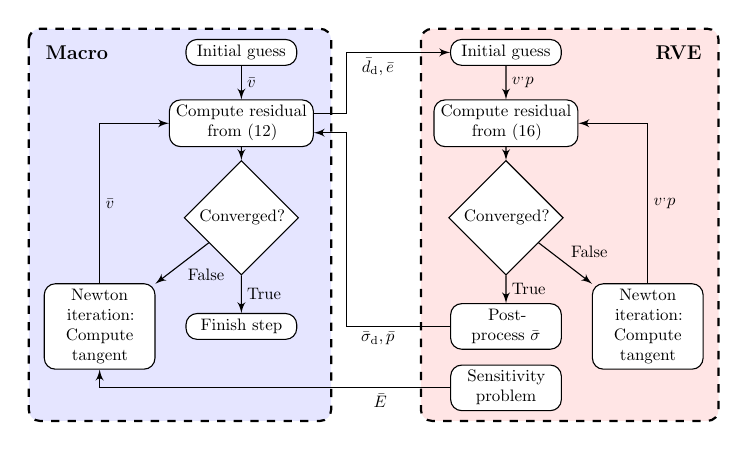
\begin{tikzpicture}[node distance = 2cm, auto,scale=0.6, transform shape]
    %\small
    %\tikzstyle{every node}=[font=\footnotesize]
    \tikzstyle{group}    = [rectangle, draw, thick, dashed, text width=6em, text centered, rounded corners]
    \tikzstyle{decision} = [diamond,   draw, fill=white, text width=6em, text centered, node distance=2.5cm, inner sep=0pt]
    \tikzstyle{block}    = [rectangle, draw, fill=white, text width=6em, text centered, rounded corners]
    \tikzstyle{line}     = [draw, -latex']

    \draw [thick, dashed, fill=blue!10, rounded corners] (-4.5,0.5) rectangle ( 1.9,-7.8);
    \draw [thick, dashed, fill=red!10,  rounded corners] ( 3.8,0.5) rectangle (10.1,-7.8);
    \node [below right, inner sep=10pt] at (-4.5,0.5) { \textbf{\large Macro} };
    \node [below left,  inner sep=10pt] at (10.1,0.5) { \textbf{\large RVE} };

    % Place nodes
    \node [block] (init) {Initial guess};
    \node [block, below of=init, text width=8em, node distance=1.5cm] (residual) {Compute residual from (12)};
    \node [decision, below of=residual,node distance=2cm] (convergence) {Converged?};
    \node [block, below of=convergence, node distance=2.3cm] (stop) {Finish step};
    \node [block, left of=stop, node distance=3cm] (update) {Newton iteration: Compute tangent};
    % Draw edges
    \path [line] (init) -- (residual) node[midway] {$\bar{\ta{v}}$};
    \path [line] (residual) -- (convergence);
    \path [line] (convergence) -- node {False} (update);
    \path [line] (convergence) -- node {True} (stop);
    \path [line] (update) |- node[near start,right] {$\bar{\ta{v}}$} (residual);

    % Place nodes
    \node [block, right of=init, node distance=5.6cm] (rve_init) {Initial guess};
    \node [block, below of=rve_init, text width=8em, node distance=1.5cm] (rve_residual) {Compute residual from (16)};
    \node [decision, below of=rve_residual, node distance=2cm] (rve_convergence) {Converged?};
    \node [block, below of=rve_convergence, node distance=2.3cm] (rve_stop) {Post-process $\bar{\ts\sigma}$};
    \node [block, right of=rve_stop, node distance=3cm] (rve_update) {Newton iteration: Compute tangent};
    % Sensitivity problem
    \node [block, below of=rve_stop, node distance=1.3cm] (rve_sensitivity) {Sensitivity problem};
    
    % Draw edges
    \path [line] (rve_init) -- (rve_residual) node[midway] {$\ta{v}^\fluct,p$};
    \path [line] (rve_residual) -- (rve_convergence);
    \path [line] (rve_convergence) -- node {False} (rve_update);
    \path [line] (rve_convergence) -- node {True} (rve_stop);
    \path [line] (rve_update) |- node[right, near start] {$\ta{v}^\fluct,p$} (rve_residual);

    \path [line] (residual.east) ++(0, 0.2cm) -- ++(0.7cm,0) |- node [below,pos=0.65] {$\bar{\ts d}_\dev, \bar{e}$} (rve_init);
    % Draw this backwards in order to get exact alignments
    \path [line, latex'-] (residual.east) ++(0,-0.2cm) -- ++(0.7cm,0) |- node [below,pos=0.65] {$\bar{\ts\sigma}_\dev, \bar{p}$} (rve_stop);

    \path [line] (rve_sensitivity) -| node[below, pos=0.10] {$\bar{\tf E}$} (update);
\end{tikzpicture}

 \end{center}
 \begin{itemize}
   \item \roughcite{\"Ohman et al. (2012) Tech. Mechanik}
 \end{itemize}

%  \begin{itemize}
%   \item[-] No free surfaces (zero porosity) $\leadsto$ Unknown subscale pressure field; singular tangent, $\ts I\dprod \bar{\tf E}\dprod \ts I\to \infty$
%   \item[-] Requires new macroscopic formulation
%  \end{itemize}
\end{frame}



%%%%%%%%%%%%%%%%%%%%%%%%%%%%%%%%%%%%%%%%%%%%%%%%%%%%%%%%%%%%%%%%%%%%%%%%%%%%%%%%%%%%%%%%%%%%%%%%%%%
\subsection{Mixed formulation}
\begin{frame}
 \frametitle{Mixed macroscale problem}
\begin{itemize}
 \item Allows for seamless transition compressibility $\to$ incompressibility
 \item Macroscale equations representing momentum balance and weak format of $\bar{e} = \bar{\ta v}\cdot\diff$
 \item Macroscale pressure $\bar{p}$ is a Lagrange multiplier
 \item Solve for $(\bar{\ta v}, \bar{p}) \in \bar{\set{V}}\times\bar{\set{P}}$ that solve the system
\end{itemize}
\begin{alignat*}{3}
 &\int_\Omega {\color{blue}\bar{\ts\sigma}_\dev\{\bar{\ts d}_\dev,\bar{p}\}} \dprod [\delta\bar{\ta v}\outerp \diff] \dif v + \int_\Omega -\bar{p}\;[\delta\bar{\ta v}\cdot\diff]\dif v &&= 0 &\quad& \forall \delta\bar{\ta v}\in \bar{\set{V}}^0\\
 &\int_\Omega \left[ {\color{blue}\bar{e}\{\bar{\ts d}_\dev,\bar{p}\}} - \bar{\ta v}\cdot\diff\right]\delta\bar{p} \dif v &&= 0&\quad& \forall \delta\bar{p}\in \bar{\set{P}}
\end{alignat*}
\begin{itemize}
 \item Can be obtained by switching control of $\bar{e} \leftrightarrow \bar{p}$ or by deriving the variationally consistent forms directly
 \item Uses standard Taylor-Hood interpolation
\end{itemize}


% \begin{align*}
%  \bar{\ts\sigma}_\dev = \frac{1}{|\Omega_\Box|} \int_{\Gamma_\Box} \ta t \outerp [\ta x - \bar{\ta x}]\dif v + \bar{p}\ts I
% \end{align*}
\end{frame}


%%%%%%%%%%%%%%%%%%%%%%%%%%%%%%%%%%%%%%%%%%%%%%%%%%%%%%%%%%%%%%%%%%%%%%%%%%%%%%%%%%%%%%%%%%%%%%%%%%%
\begin{frame}
 \frametitle{FE\textsuperscript{2} format: Mixed macroscale equation}
%  \begin{itemize}
%   \item Introduce macroscale pressure $\bar{p}$ as independent variable, impose identity $\bar{e} = \bar{\ta v}\cdot \diff$ in a weak sense
%  \end{itemize}
% 
%  \begin{itemize}
%   \item Macroscale-problem (mixed format)
%   \begin{itemize}
%    \item Fields: $\bar{\ta v}$, $\bar{p}$%, solved from  \eqref{eq:new_macro}
%   \end{itemize}
%   \item RVE-problem: $\bar{\ts d}_\dev, \bar{p} \longrightarrow \bar{\ts\sigma}_\dev, \bar{e}$
%   \begin{itemize}
%    \item Input: $\bar{\ts d}_\dev$, $\bar{p}$
%    \item Fields: $\ta v^\fluct$, $p$, $\bar{e}$%, solved from \eqref{eq:rve_problem_new}
%    \item Output: $\bar{\ts\sigma}_\dev$ (post-processed), $\bar{e}$
%   \end{itemize}
%  \end{itemize}
% 
%  \begin{itemize}
%   \item Valid for seamless transition from compressible to incompressible macroscale response ($\bar{e}\to 0$ instead of $\bar{p}\to\infty$).
%  \end{itemize}

 \begin{center}
 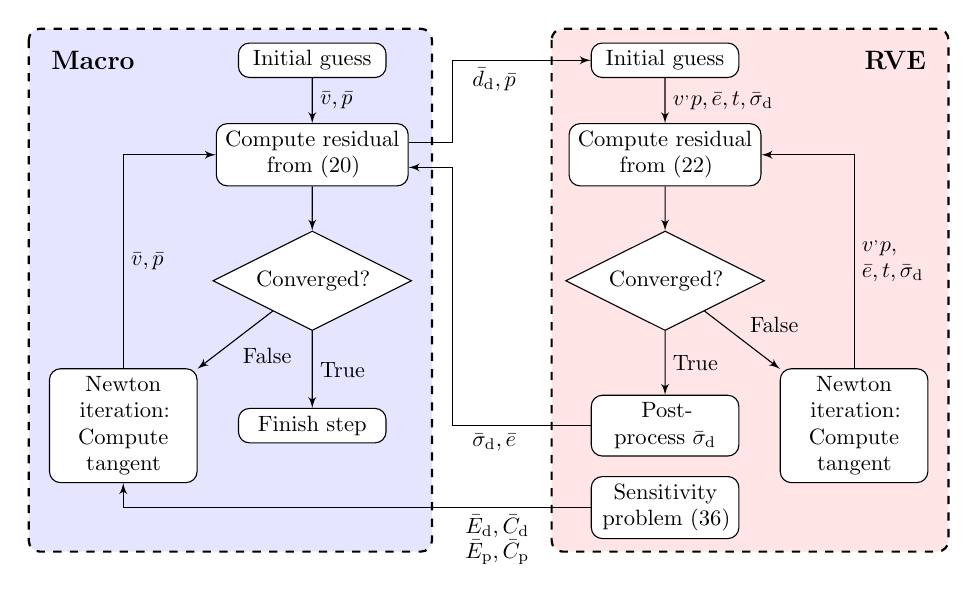
\begin{tikzpicture}[node distance = 2cm, auto,scale=0.8, transform shape, >=latex']
    %\small
    %\tikzstyle{every node}=[font=\footnotesize]
    \tikzstyle{group}    = [rectangle, draw, thick, dashed, text width=6em, text centered, rounded corners]
    \tikzstyle{decision} = [diamond,   draw, fill=white, text width=6em, text centered, aspect=2, node distance=2.5cm, inner sep=2pt]
    \tikzstyle{block}    = [rectangle, draw, fill=white, text width=6em, text centered, rounded corners]
    \tikzstyle{line}     = [draw, ->]

    \draw [thick, dashed, fill=blue!10, rounded corners] (-4.5,0.5) rectangle ( 1.9,-7.8);
    \draw [thick, dashed, fill=red!10,  rounded corners] ( 3.8,0.5) rectangle (10.1,-7.8);
    \node [below right, inner sep=10pt] at (-4.5,0.5) { \textbf{\large Macro} };
    \node [below left,  inner sep=10pt] at (10.1,0.5) { \textbf{\large RVE} };

    % Place nodes
    \node [block] (init) {Initial guess};
    \node [block, below of=init, text width=8em, node distance=1.5cm] (residual) {Compute residual from (20)};
    \node [decision, below of=residual,node distance=2cm] (convergence) {Converged?};
    \node [block, below of=convergence, node distance=2.3cm] (stop) {Finish step};
    \node [block, left of=stop, node distance=3cm] (update) {Newton iteration: Compute tangent};
    % Draw edges
    \path [line] (init) -- (residual) node[midway] {$\bar{\ta{v}},\bar{p}$};
    \path [line] (residual) -- (convergence);
    \path [line] (convergence) -- node {False} (update);
    \path [line] (convergence) -- node {True} (stop);
    \path [line] (update) |- node[near start,right] {$\bar{\ta{v}},\bar{p}$} (residual);

    % Place nodes
    \node [block, right of=init, node distance=5.6cm] (rve_init) {Initial guess};
    \node [block, below of=rve_init, text width=8em, node distance=1.5cm] (rve_residual) {Compute residual from (22)};
    \node [decision, below of=rve_residual, node distance=2cm] (rve_convergence) {Converged?};
    \node [block, below of=rve_convergence, node distance=2.3cm] (rve_stop) {Post-process $\bar{\ts\sigma}_\dev$};
    \node [block, right of=rve_stop, node distance=3cm] (rve_update) {Newton iteration: Compute tangent};
    % Sensitivity problem
    \node [block, below of=rve_stop, node distance=1.3cm] (rve_sensitivity) {Sensitivity problem (36)};
    
    % Draw edges
    \path [line] (rve_init) -- (rve_residual) node[midway] {$\ta{v}^\fluct,p, \bar{e}, \ta t, \bar{\ts\sigma}_\dev$};
    \path [line] (rve_residual) -- (rve_convergence);
    \path [line] (rve_convergence) -- node {False} (rve_update);
    \path [line] (rve_convergence) -- node {True} (rve_stop);
    \path [line] (rve_update) |- node[right, near start, text width=1.5em] {$\ta{v}^\fluct,p$, $\bar{e}, \ta t, \bar{\ts\sigma}_\dev$} (rve_residual);

    \path [line] (residual.east) ++(0, 0.2cm) -- ++(0.7cm,0) |- node [below,pos=0.65] {$\bar{\ts d}_\dev, \bar{p}$} (rve_init);
    % Draw this backwards in order to get exact alignments
    \path [line, <-] (residual.east) ++(0,-0.2cm) -- ++(0.7cm,0) |- node [below,pos=0.65] {$\bar{\ts\sigma}_\dev, \bar{e}$} (rve_stop);

    \path [line] (rve_sensitivity) -| node[below, pos=0.10] {$\substack{\displaystyle\bar{\tf E}_\ded,\bar{\ts C}_\ded \\ \displaystyle\bar{\ts E}_\dep,\bar{C}_\dep}$} (update);
\end{tikzpicture}

 \end{center}
\vspace{-6truemm}
 \begin{itemize}
   \item \roughcite{\"Ohman et al. (2013) Comput. Methods Appl. Mech. Engrg. (In press)}
 \end{itemize}

\end{frame}


%%%%%%%%%%%%%%%%%%%%%%%%%%%%%%%%%%%%%%%%%%%%%%%%%%%%%%%%%%%%%%%%%%%%%%%%%%%%%%%%%%%%%%%%%%%%%%%%%%%
\begin{frame}
\frametitle{RVE-problem for mixed control: Dirichlet b.c.}
 \begin{itemize}
  \item Dirichlet b.c: $\ta v^\fluct = \ta 0$ on $\Gamma_\Box$ with $\ta v = \ta v^\macro_\dev + \ta v^\macro_\vol + \ta v^\fluct$
  \item For given macroscale variables $\bar{\ts d}_\dev$ and $\bar p$, find ($\ta v^\fluct,p,\bar{e})\in\set{V}_\Box^{\Dirichlet,0}\times\set{P}_\Box\times\set{R}$ that solve the system
 \end{itemize}
\vspace{-2truemm}
\begin{alignat*}{4}
    & a_\Box(\ta{v};\delta \ta{v}^\fluct) +  b_\Box(p,\delta\ta{v}^\fluct)
    && =
    l^\pore_\Box(\delta \ta{v}^\fluct)
    &\quad& \forall\; \delta \ta{v}^\fluct &&\in \set{V}_\Box^{\Dirichlet,0}
 \\
    &b_\Box(\delta p, \ta{v})
    && =
    0
    && \forall\; \delta p &&\in \set{P}_\Box
\\
    &\color{red}b_\Box(p,\ta{x}_\mean)\delta\bar{e}
    &&\color{red} =
    [l_\Box^\pore(\ta{x}_\mean) - \bar{p}]\delta\bar{e}
    &&\color{red} \forall\; \delta\bar{e} &&\color{red}\in \set{R}
\end{alignat*}
\vspace{-5truemm}
\begin{align*}
    a_\Box(\ta{v};\delta \ta{v})
    & \defeq
    %\langle\ta{\sigma}_\dev(\ta{d}) : \delta \ta{d}\rangle_{\Box} =
    \frac{1}{|\Omega_\Box|}\int_{\Omega^\particle_\Box} \ta{\sigma}_\dev(\ta{d}) \dprod \left[\delta \ta{v} \outerp \diff\right] \dif v
\\
    b_\Box(p, \ta{v})
    & \defeq
    %\langle -p\ta{I} \dprod \ta{d}\rangle_{\Box} =
    \frac{1}{|\Omega_\Box|}\int_{\Omega^\particle_\Box} -p\;[\ta{v}\cdot \diff] \dif v
\\
    l_\Box(\delta \ta{v})
    & \defeq
    %\frac{1}{|\Omega_{\Box}|} \int_{\Gamma_{\Box}^\pore} \hat{\ts\sigma}\dprod\left[\delta\ta{v}\outerp\hat{\diff}\right] \dif a =
    \frac{1}{|\Omega_{\Box}|} \int_{\Gamma_{\Box}^\pore}
  \gamma_\surf\left[\delta\ta{v}\cdot\hat{\ta\nabla}\right] \dif a
\end{align*}
\begin{gather*}
 \ta v_\dev^\macro \defeq \bar{\ts d}_\dev \cdot[\ta x - \bar{\ta x}], \quad \ta v_\vol^\macro \defeq \bar{e}\,\ta x_\mean,\quad \ta{x}_\mean \defeq \frac13[\ta x-\bar{\ta x}], \quad \bar{\ta x} = \text{RVE center}
\end{gather*}
\end{frame}


%%%%%%%%%%%%%%%%%%%%%%%%%%%%%%%%%%%%%%%%%%%%%%%%%%%%%%%%%%%%%%%%%%%%%%%%%%%%%%%%%%%%%%%%%%%%%%%%%%%
\begin{frame}
\frametitle{RVE-problem for mixed control: Neumann b.c.}
 \begin{itemize}
  \item Neumann b.c: $\ts\sigma\cdot\ta n = \bar{\ts\sigma}\cdot\ta n$ on $\Gamma_\Box$
  \item For given macroscale variables $\bar{\ts d}_\dev$ and $\bar p$, find ($\ta{v},p,\bar{\ts\sigma}_\dev)\in\times\set{V}_\Box\times\set{P}_\Box\times\set{R}_\dev^{3\times3}$ that solve the system
 \end{itemize}
\vspace{-2truemm}
\begin{alignat*}{4}
    & a_\Box(\ta{v};\delta \ta{v}) +  b_\Box(p,\delta\ta{v}) + {\color{red}c_\Box(\bar{\ts\sigma}_\dev, \delta\ta v)}
    && =
    {\color{red}f_\Box(\bar{p},\delta\ta v)} + l^\pore_\Box(\delta \ta{v})
    \;\forall\; \delta \ta{v} \in \set{V}_\Box
 \\
    &b_\Box(\delta p, \ta{v})
    && =
    0
    \qquad\qquad\qquad\qquad\;\;\forall\; \delta p \in \set{P}_\Box
\\
    &\color{red}c_\Box(\delta\bar{\ts\sigma}_\dev, \ta v)
    && \color{red}=
    -\bar{\ts d}_\dev \dprod \delta\bar{\ts\sigma}_\dev
    \;\;\;\forall\; \delta\bar{\ts\sigma}_\dev \in \set{R}^{3\times 3}_\dev
\end{alignat*}
\vspace{-5truemm}
\begin{itemize}
 \item Expressed in deviatoric base-dyads $\ts E_i$:
\end{itemize}
\begin{alignat*}{4}
 &\color{red}c_\Box(\delta\bar{\sigma}_{\dev,i} \ts E_i, \ta v) &&\color{red}= -\bar{d}_{\dev,i} \delta\bar{\sigma}_{\dev,i}
&\quad\quad& \color{red}\forall\; \delta\bar{\sigma}_{\dev,i} &&\color{red}\in \set{R}
\end{alignat*}
\begin{align*}
    f_\Box(\bar{p};\ta{v}) & \defeq -\frac{1}{|\Omega_\Box|} \int_{\Gamma_\Box} [\ta v\cdot\ta n]\dif A \,\bar{p}
\\
    c_\Box(\bar{\ts\sigma}_\dev, \ta v) & \defeq -\frac{1}{|\Omega_\Box|} \int_{\Gamma_\Box} [\ta v\outerp\ta n]_\dev \dif A\dprod \bar{\ts\sigma}_\dev
\end{align*}
\end{frame}

%%%%%%%%%%%%%%%%%%%%%%%%%%%%%%%%%%%%%%%%%%%%%%%%%%%%%%%%%%%%%%%%%%%%%%%%%%%%%%%%%%%%%%%%%%%%%%%%%%%
\begin{frame}
\frametitle{RVE-problem for mixed control: Periodicity b.c.}
 \begin{itemize}
  \item Periodic b.c: $ \jump{\ta v^\fluct} = \ta 0$ on $\Gamma_\Box$ with $\ta v = \ta v^\macro_\dev + \ta v^\macro_\vol + \ta v^\fluct$ 
  \item For given macroscale variables $\bar{\ts d}_\dev$ and $\bar p$, find $(\ta v, p, \ta t, \bar{e}) \in\set{V}_\Box\times\set{P}_\Box\times\set{T}_\Box\times\set{R}$ that solve the system
 \end{itemize}
\vspace{-2truemm}
\begin{align*}
 &a_\Box(\ta v; \delta\ta v) + b_\Box(p,\delta\ta v) {\color{red}- t_\Box(\ta t,\delta\ta v)} &&= l_\Box(\delta\ta v)
&&\forall\;\delta\ta v\in \set{V}_\Box
\\
 &b_\Box(\delta p, \ta v) &&= 0
&&\forall\;\delta p\in\set{P}_\Box
\\
 &{\color{red}t_\Box(\delta\ta t, \bar{e}\;\ta x_\mean - \ta v)} &&{\color{red} = -t_\Box(\delta\ta t, \bar{\ts d}_\dev\cdot[\ta x-\bar{\ta x}])}
&&{\color{red}\forall\;\delta\ta t\in\set{T}_\Box}
\\
 &{\color{red}t_\Box(\ta t, \ta x_\mean) \delta\bar{e}} &&{\color{red}= -\bar p\;\delta\bar{e} }
&&{\color{red}\forall\;\delta\bar{e}\in\set{R}}
\end{align*}

\vspace{-5truemm}
\begin{align*}
 t_\Box(\ta t, \ta v) &\defeq \frac{1}{|\Omega_\Box|}\int_{\Gamma_\Box^+} \ta t \cdot \jump{\ta v} \dif a
\end{align*}
\begin{itemize}
  \item Jump $\jump{\bullet} \defeq \bullet^+ - \bullet^-$, $\Gamma_\Box^+ =$ positive sides of cubic RVE
\end{itemize}
\end{frame}

%%%%%%%%%%%%%%%%%%%%%%%%%%%%%%%%%%%%%%%%%%%%%%%%%%%%%%%%%%%%%%%%%%%%%%%%%%%%%%%%%%%%%%%%%%%%%%%%%%%
\section{Results}
\begin{frame}
 \frametitle{FE\textsuperscript{2} -- Dirichlet b.c.}
 \movie[width=\linewidth,poster]{\includegraphics[width=\linewidth]{figures/macro_fe2_0000}}{macro_fe2_slow.wmv}
 %\includegraphics[width=\linewidth]{figures/macro_fe2_0000}
\end{frame}

%%%%%%%%%%%%%%%%%%%%%%%%%%%%%%%%%%%%%%%%%%%%%%%%%%%%%%%%%%%%%%%%%%%%%%%%%%%%%%%%%%%%%%%%%%%%%%%%%%%
\begin{frame}
 \frametitle{RVE behavior -- Free sintering, $\bar{\ts\sigma} = \ts 0$}
 \begin{tikzpicture}
  \node at (0,0) {\includegraphics[scale=0.15]{figures/initial_rve}};
  \node at (4,2) {\includegraphics[scale=0.15]{figures/final_dirichlet}};
  \node at (4,-2) {\includegraphics[scale=0.15]{figures/final_neumann}};
  \node at (0,1.5) {Initial};
  \node at (4,3.5) {Dirichlet};
  \node at (4,-0.5) {Neumann};
  \draw[-latex] (1.5,0.5) -- (2.5,1);
  \draw[-latex] (1.5,-0.5) -- (2.5,-1);
  \node at (8,2) {\includegraphics[scale=0.2]{figures/rve_dirichlet_2}};
  \node at (8,-2) {\includegraphics[scale=0.2]{figures/rve_neumann_2}};
 \end{tikzpicture}
\end{frame}

%%%%%%%%%%%%%%%%%%%%%%%%%%%%%%%%%%%%%%%%%%%%%%%%%%%%%%%%%%%%%%%%%%%%%%%%%%%%%%%%%%%%%%%%%%%%%%%%%%%
\begin{frame}
\begin{tikzpicture}
 \frametitle{Macroscopic response -- Free sintering}
 \begin{axis}[
    width=1.0\linewidth,
    height=0.6\linewidth,
    ylabel={Relative density [\%]},xlabel={Time (scaled)},
    xmax=1, xmin=0, ymax=1.01, ymin=0.83,
    cycle list name=linestyles,
    yticklabel style={font=\tiny}, xticklabel style={font=\tiny},
%     scaled y ticks=manual:{}{\pgfmathparse{#1*100}}, % Scale for percentage
%     scaled x ticks=manual:{}{\pgfmathparse{#1*1000}}, % Scale for percentage
    legend style={draw=black,rounded corners=3pt,font=\footnotesize},
    legend pos=south east
    ]
  \addplot[blue ,densely dashed] table[y index=2] {figures/macro_3_dirichlet_x.out.matdata};
  \addlegendentry {Dirichlet 3$\times$3}
  \addplot[red  ,densely dashed] table[y index=2] {figures/macro_2_dirichlet_x.out.matdata};
  \addlegendentry {Dirichlet 2$\times$2}
  \addplot[black,densely dashed] table[y index=2] {figures/macro_1_dirichlet_x.out.matdata};
  \addlegendentry {Dirichlet 1$\times$1}

  \addplot[blue ] table[y index=2] {figures/macro_3_neumann_x.out.matdata};
  \addlegendentry {Neumann 3$\times$3}
  \addplot[red  ] table[y index=2] {figures/macro_2_neumann_x.out.matdata};
  \addlegendentry {Neumann 2$\times$2}
  \addplot[black] table[y index=2] {figures/macro_1_neumann_x.out.matdata};
  \addlegendentry {Neumann 1$\times$1}
 \end{axis}
\end{tikzpicture}
 \vspace{-5truemm}
 \begin{itemize}
  \item ``Stiff'' WC-particles in ``compliant'' Co-matrix $\to$ Neumann b.c. has superior convergence.
 \end{itemize}

\end{frame}

% %%%%%%%%%%%%%%%%%%%%%%%%%%%%%%%%%%%%%%%%%%%%%%%%%%%%%%%%%%%%%%%%%%%%%%%%%%%%%%%%%%%%%%%%%%%%%%%%%%%
% \begin{frame}
%  \frametitle{RVE -- Elasticity}
%   
% \end{frame}

%%%%%%%%%%%%%%%%%%%%%%%%%%%%%%%%%%%%%%%%%%%%%%%%%%%%%%%%%%%%%%%%%%%%%%%%%%%%%%%%%%%%%%%%%%%%%%%%%%%
\begin{frame}
 \frametitle{Concluding remarks and Outlook}
 \begin{itemize}
  \item So far (\roughcite{\"Ohman et al. (2013) Comput. Methods Appl. Mech. Engrg. (In press)})

  \begin{itemize}
   \item Framework for seamless transition to macroscopic incompressibility
   \item Variationally consistent upscaling of fine-scale equations (not discussed here)
   \item Code available in OOFEM  \url{http://www.oofem.org/}
  \end{itemize}
  \item Current work: Incompressible elasticity
 \end{itemize}
 \begin{center}
  \includegraphics[width=0.25\textwidth]{figures/elastic_dirichlet.png}
  \includegraphics[width=0.25\textwidth]{figures/elastic_neumann.png}
  \includegraphics[width=0.25\textwidth]{figures/elastic_periodic3.png}
 \end{center}
\end{frame}


%%%%%%%%%%%%%%%%%%%%%%%%%%%%%%%%%%%%%%%%%%%%%%%%%%%%%%%%%%%%%%%%%%%%%%%%%%%%%%%%%%%%%%%%%%%%%%%%%%%
% \section{Implementation}
% \begin{frame}
%  \frametitle{Dirichlet b.c. implementation --- Issues}
%  \begin{itemize}
%   \item Inconvenient equation of $\bar{e}$. Unknown is global to the RVE problem (single unknown on the entire boundary). Where should it belong?
%   \item Velocity fluctuations $\ta v^\fluct$ would require an alternative Stokes' flow-formulation.
%   \item How should one deal with 
% \begin{equation*}
%     b_\Box(p,\ta{x}_\mean)\delta\bar{e}
%      =
%     [l_\Box^\pore(\ta{x}_\mean) - \bar{p}]\delta\bar{e}
%     \quad \forall\; \delta\bar{e} \in \set{R}
% \end{equation*}
%   which connects elements to this global test-function $\delta\bar{e}$ ? 
%  \end{itemize}
% \end{frame}
% 
% \begin{frame}
% \frametitle{Dirichlet b.c. implementation --- Solutions}
% \begin{itemize}
%   \item Introduce internal DOFs into boundary conditions. OOFEM numbers them along with everything else.
%   \item OOFEM already support slave DOFs! Simply use 
%   \begin{equation*}
%    \ta v = \overbrace{\underbrace{\bar{\ts d}_\dev}_{\text{Prescribed}} \cdot \underbrace{[\ta x - \bar{\ta x}]}_{\text{Weights}}}^{\ta v^\macro_\dev} + 
%            \overbrace{\underbrace{\bar{e}}_{\text{Unknown}} \underbrace{\frac13 [\ta x - \bar{\ta x}]}_{\text{Weight}}}^{\ta v^\macro_\vol}  \quad\text{on } \Gamma_\Box
%   \end{equation*}
%   ( only boundary matters, internal DOFs can left alone )
%   \item Nothing else to do. OOFEMs slave DOF transformations takes care of the third equation.
%   \item Better yet, $\bar{\ts\sigma}_\dev$ is obtained trivially as the reaction-forces associated with the prescribed $\bar{\ts d}_\dev$-DOFs!
%   \item Implemented in \texttt{MixedGradientPressureDirichlet}
%  \end{itemize}
% \end{frame}
% 
% %%%%%%%%%%%%%%%%%%%%%%%%%%%%%%%%%%%%%%%%%%%%%%%%%%%%%%%%%%%%%%%%%%%%%%%%%%%%%%%%%%%%%%%%%%%%%%%%%%%
% \begin{frame}
% \frametitle{Neumann b.c. implementation --- Issues}
%  \begin{itemize}
%   \item Where should the new global DOFs for $\bar{\ts\sigma}_\dev$ be stored?
%   \item How should $c_\Box(\bullet,\bullet)$ be computed?
%  \end{itemize}
% \end{frame}
% \begin{frame}
% \frametitle{Neumann b.c. implementation --- Solutions}
%  \begin{itemize}
%   \item Store $\bar{\ts\sigma}_{\dev}$ as internal DOFs in the boundary condition.
%   \item Introduce \texttt{ActiveBoundaryCondition}: Boundary condition assembles contributions to residual and tangent matrices itself.
%   \item Active b.c. stores a list of element boundaries
%   \item Common interface with Dirichlet b.c; $(\bar{\ts d}_\dev, \bar{p}) \to (\bar{\ts\sigma}_\dev,\bar{e})$
%   \item Implemented in \texttt{MixedGradientPressureNeumann}
%  \end{itemize}
% \end{frame}
% 
% \begin{frame}
%  \frametitle{FE\textsuperscript{2} Implementation}
%  \begin{itemize}
%   \item \texttt{FE2FluidMaterial} solves RVE-problem in each integration point.
%   \item Benefit from OO-design:\\
%  \begin{center}
%  \includegraphics[width=0.7\linewidth]{figures/mixedgradientpressurebc.png}
%   \end{center}
%   \item Expects first boundary condition on RVE to be of the type \texttt{MixedGradientPressureBC}
%   \item Also implemented are the necessary tangents (4 of them!)
%   \begin{align*}
%    \pd{\bar{\ts\sigma}_\dev}{\bar{\ts d}_\dev} \qquad
%    \pd{\bar{\ts\sigma}_\dev}{\bar{p}} \qquad
%    \pd{\bar{e}}{\bar{\ts d}_\dev} \qquad
%    \pd{\bar{e}}{\bar{p}}
%   \end{align*}
%  \item Fluid material with memory; have to track integration points.
%  \end{itemize}
% 
% \end{frame}
% 
% 
% %%%%%%%%%%%%%%%%%%%%%%%%%%%%%%%%%%%%%%%%%%%%%%%%%%%%%%%%%%%%%%%%%%%%%%%%%%%%%%%%%%%%%%%%%%%%%%%%%%%
% \begin{frame}
% \frametitle{The final pieces}
%  \begin{itemize}
%   \item Large toplogical changes requires remeshing
%   \begin{itemize}
%   \item Added Triangle bindings (\roughcite{J. Schewchuck})
%   \item Topology-tracker: Points tracking surface geometry
%   \item Mesh quality ``error''-estimator to determine when to re-mesh.
%   \end{itemize}
%  \item Surface tension loading implemented as an active boundary condition (should work automatically for all standard elements).
%  \end{itemize}
% \end{frame}

\end{document}
